\begin{frame}
    \frametitle{Security in Bitcoin}
    \begin{itemize}
        \item \textbf{Authentication}
            \begin{itemize}
                \item Am I paying the right person?
            \end{itemize}
        \item \textbf{Integrity}
            \begin{itemize}
                \item Is the coin double-spent?
                \item Can an attacker reverse or change transactions?
            \end{itemize}
        \item \textbf{Availability}
            \begin{itemize}
                \item Can I make a transactions anytime I want?
            \end{itemize}
        \item \textbf{Confidentiality}
            \begin{itemize}
                \item Are my transactions private? Anonymous?
            \end{itemize}
    \end{itemize}
\end{frame}

\begin{frame}
    \frametitle{Security in Bitcoin}
    \begin{itemize}
        \item \textbf{Authentication -> \alert{Public Key Crypto: Digital Signatures}}
            \begin{itemize}
                \item Am I paying the right person?
            \end{itemize}
        \item \textbf{Integrity -> \alert{Digital Signatures and Cryptographic Hash}}
            \begin{itemize}
                \item Is the coin double-spent?
                \item Can an attacker reverse or change transactions?
            \end{itemize}
        \item \textbf{Availability -> \alert{Broadcast messages to the P2P network}}
            \begin{itemize}
                \item Can I make a transactions anytime I want?
            \end{itemize}
        \item \textbf{Confidentiality -> \alert{Pesudonymity}}
            \begin{itemize}
                \item Are my transactions private? Anonymous?
            \end{itemize}
    \end{itemize}
\end{frame}

\begin{frame}
    \frametitle{Cryptographic Hash Function}
    \begin{itemize}
        \item \textbf{Computationally efficient}
        \item \textbf{Consistent} \\
            hash(x) always yields same result.
        \item \textbf{Collision Resistant} \\
            Given $hash(W) = Z$, hard to find X such that $hash(X) = Z$
        \item \textbf{One-way} \\
            Given Y, hard to find X s.t. $hash(X) = Y$
    \end{itemize}
    \begin{columns}
        \begin{column}{0.5\textwidth}
            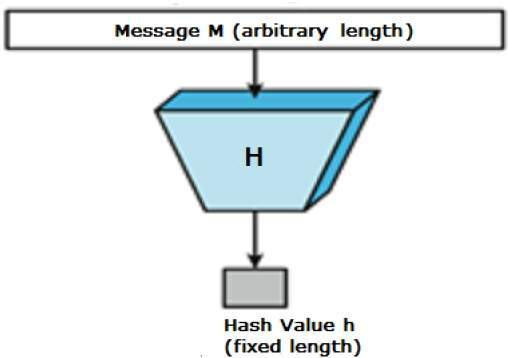
\includegraphics[scale=0.3]{./figures/hash_functions.jpg}
        \end{column}
        \begin{column}{0.5\textwidth}
            Common Hash Functions:
            \begin{itemize}
                \item \textbf{MD5}
                \item \textbf{SHA-1}
                \item \textbf{SHA-2}
                    \begin{itemize}
                        \item SHA-256
                        \item SHA-384
                        \item SHA-512
                    \end{itemize}
            \end{itemize}
        \end{column}
    \end{columns}
\end{frame}

\begin{frame}[fragile]
    \frametitle{Hash Function Example}
    \begin{lstlisting}[language=Python]
    SHA224("")
    0x d14a028c2a3a2bc9476102bb288234c415a2b01f828ea62ac5b3e42f
    SHA256("")
    0x e3b0c44298fc1c149afbf4c8996fb92427ae41e4649b934ca495991b7852b855
    \end{lstlisting}

    Even a small change in the message wil result in a mostly different hash.
    \begin{lstlisting}[language=Python]
    SHA224("The quick brown fox jumps over the lazy dog")
    0x 730e109bd7a8a32b1cb9d9a09aa2325d2430587ddbc0c38bad911525
    SHA224("The quick brown fox jumps over the lazy dog.")
    0x 619cba8e8e05826e9b8c519c0a5c68f4fb653e8a3d8aa04bb2c8cd4c
    \end{lstlisting}

    Proof of work first sight:

    Given a basic string \alert{hello world!} + random number \alert{nonce}

    We need the digest have 4 leading 0.
    \begin{lstlisting}[language=Python]
    "Hello, world!0" => 1312af178c253f84028d480a6adc1e25e81caa44c749ec81976192e2ec934c64
    "Hello, world!1" => e9afc424b79e4f6ab42d99c81156d3a17228d6e1eef4139be78e948a9332a7d8
    "Hello, world!2" => ae37343a357a8297591625e7134cbea22f5928be8ca2a32aa475cf05fd4266b7
    ...
    "Hello, world!4248" => 6e110d98b388e77e9c6f042ac6b497cec46660deef75a55ebc7cfdf65cc0b965
    "Hello, world!4249" => c004190b822f1669cac8dc37e761cb73652e7832fb814565702245cf26ebb9e6
    "Hello, world!4250" => 0000c3af42fc31103f1fdc0151fa747ff87349a4714df7cc52ea464e12dcd4e9
    \end{lstlisting}
\end{frame}

\begin{frame}
    \frametitle{Public Key Crypto: Encryption}
    Key pair: Public Key and Private Key
    \begin{columns}
        \begin{column}{0.35\textwidth}
            \begin{center}
                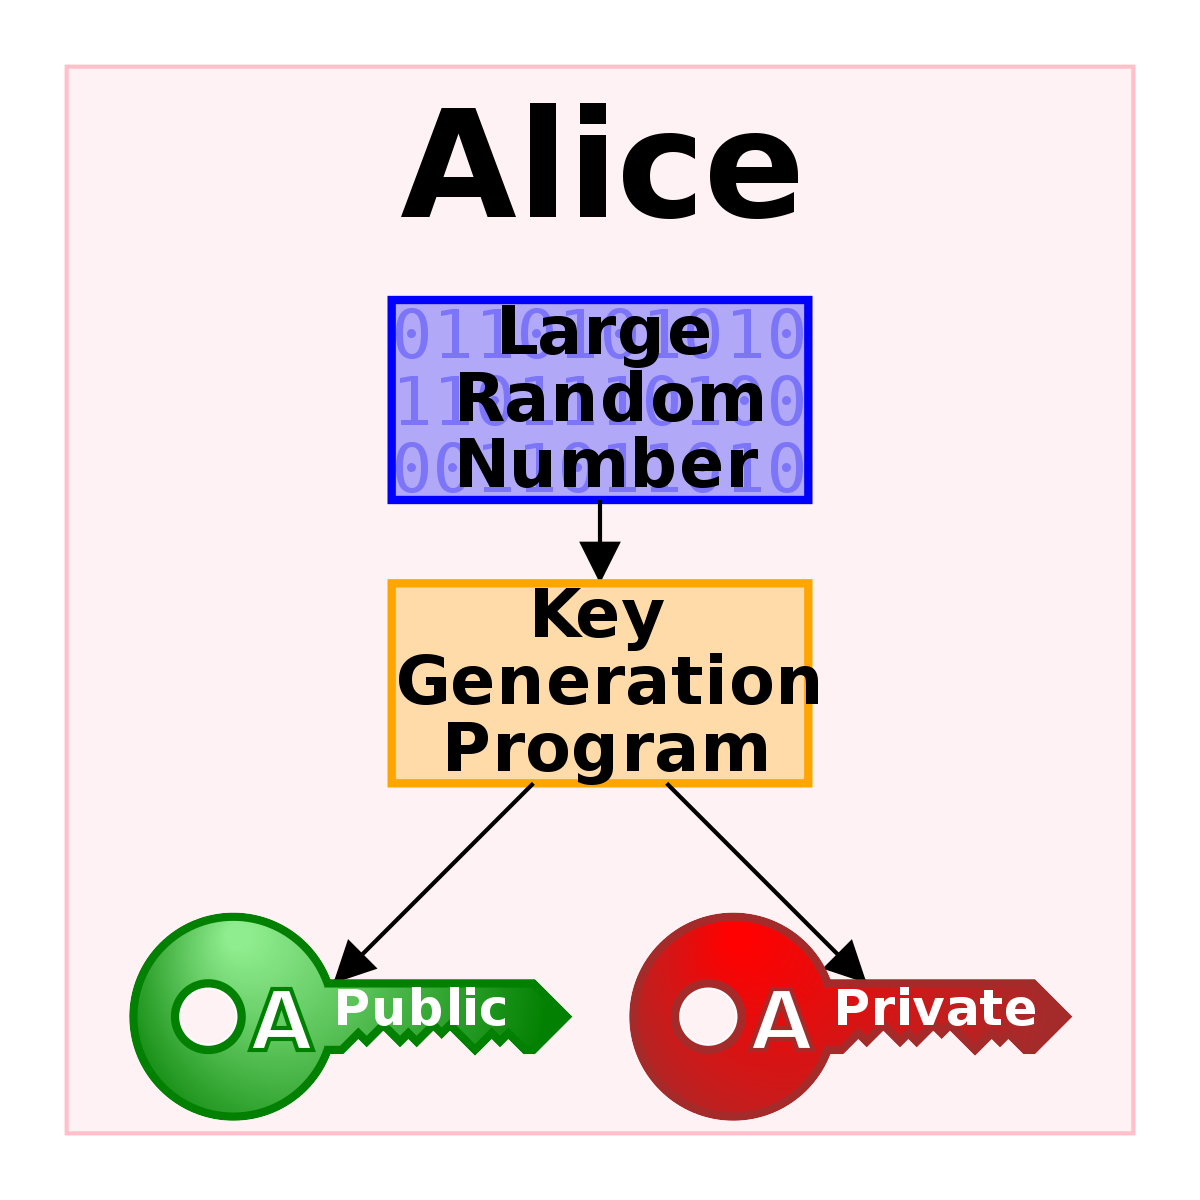
\includegraphics[scale=0.1]{./figures/Public-key-crypto.png}
            \end{center}
        \end{column}
        \begin{column}{0.65\textwidth}
            \begin{center}
                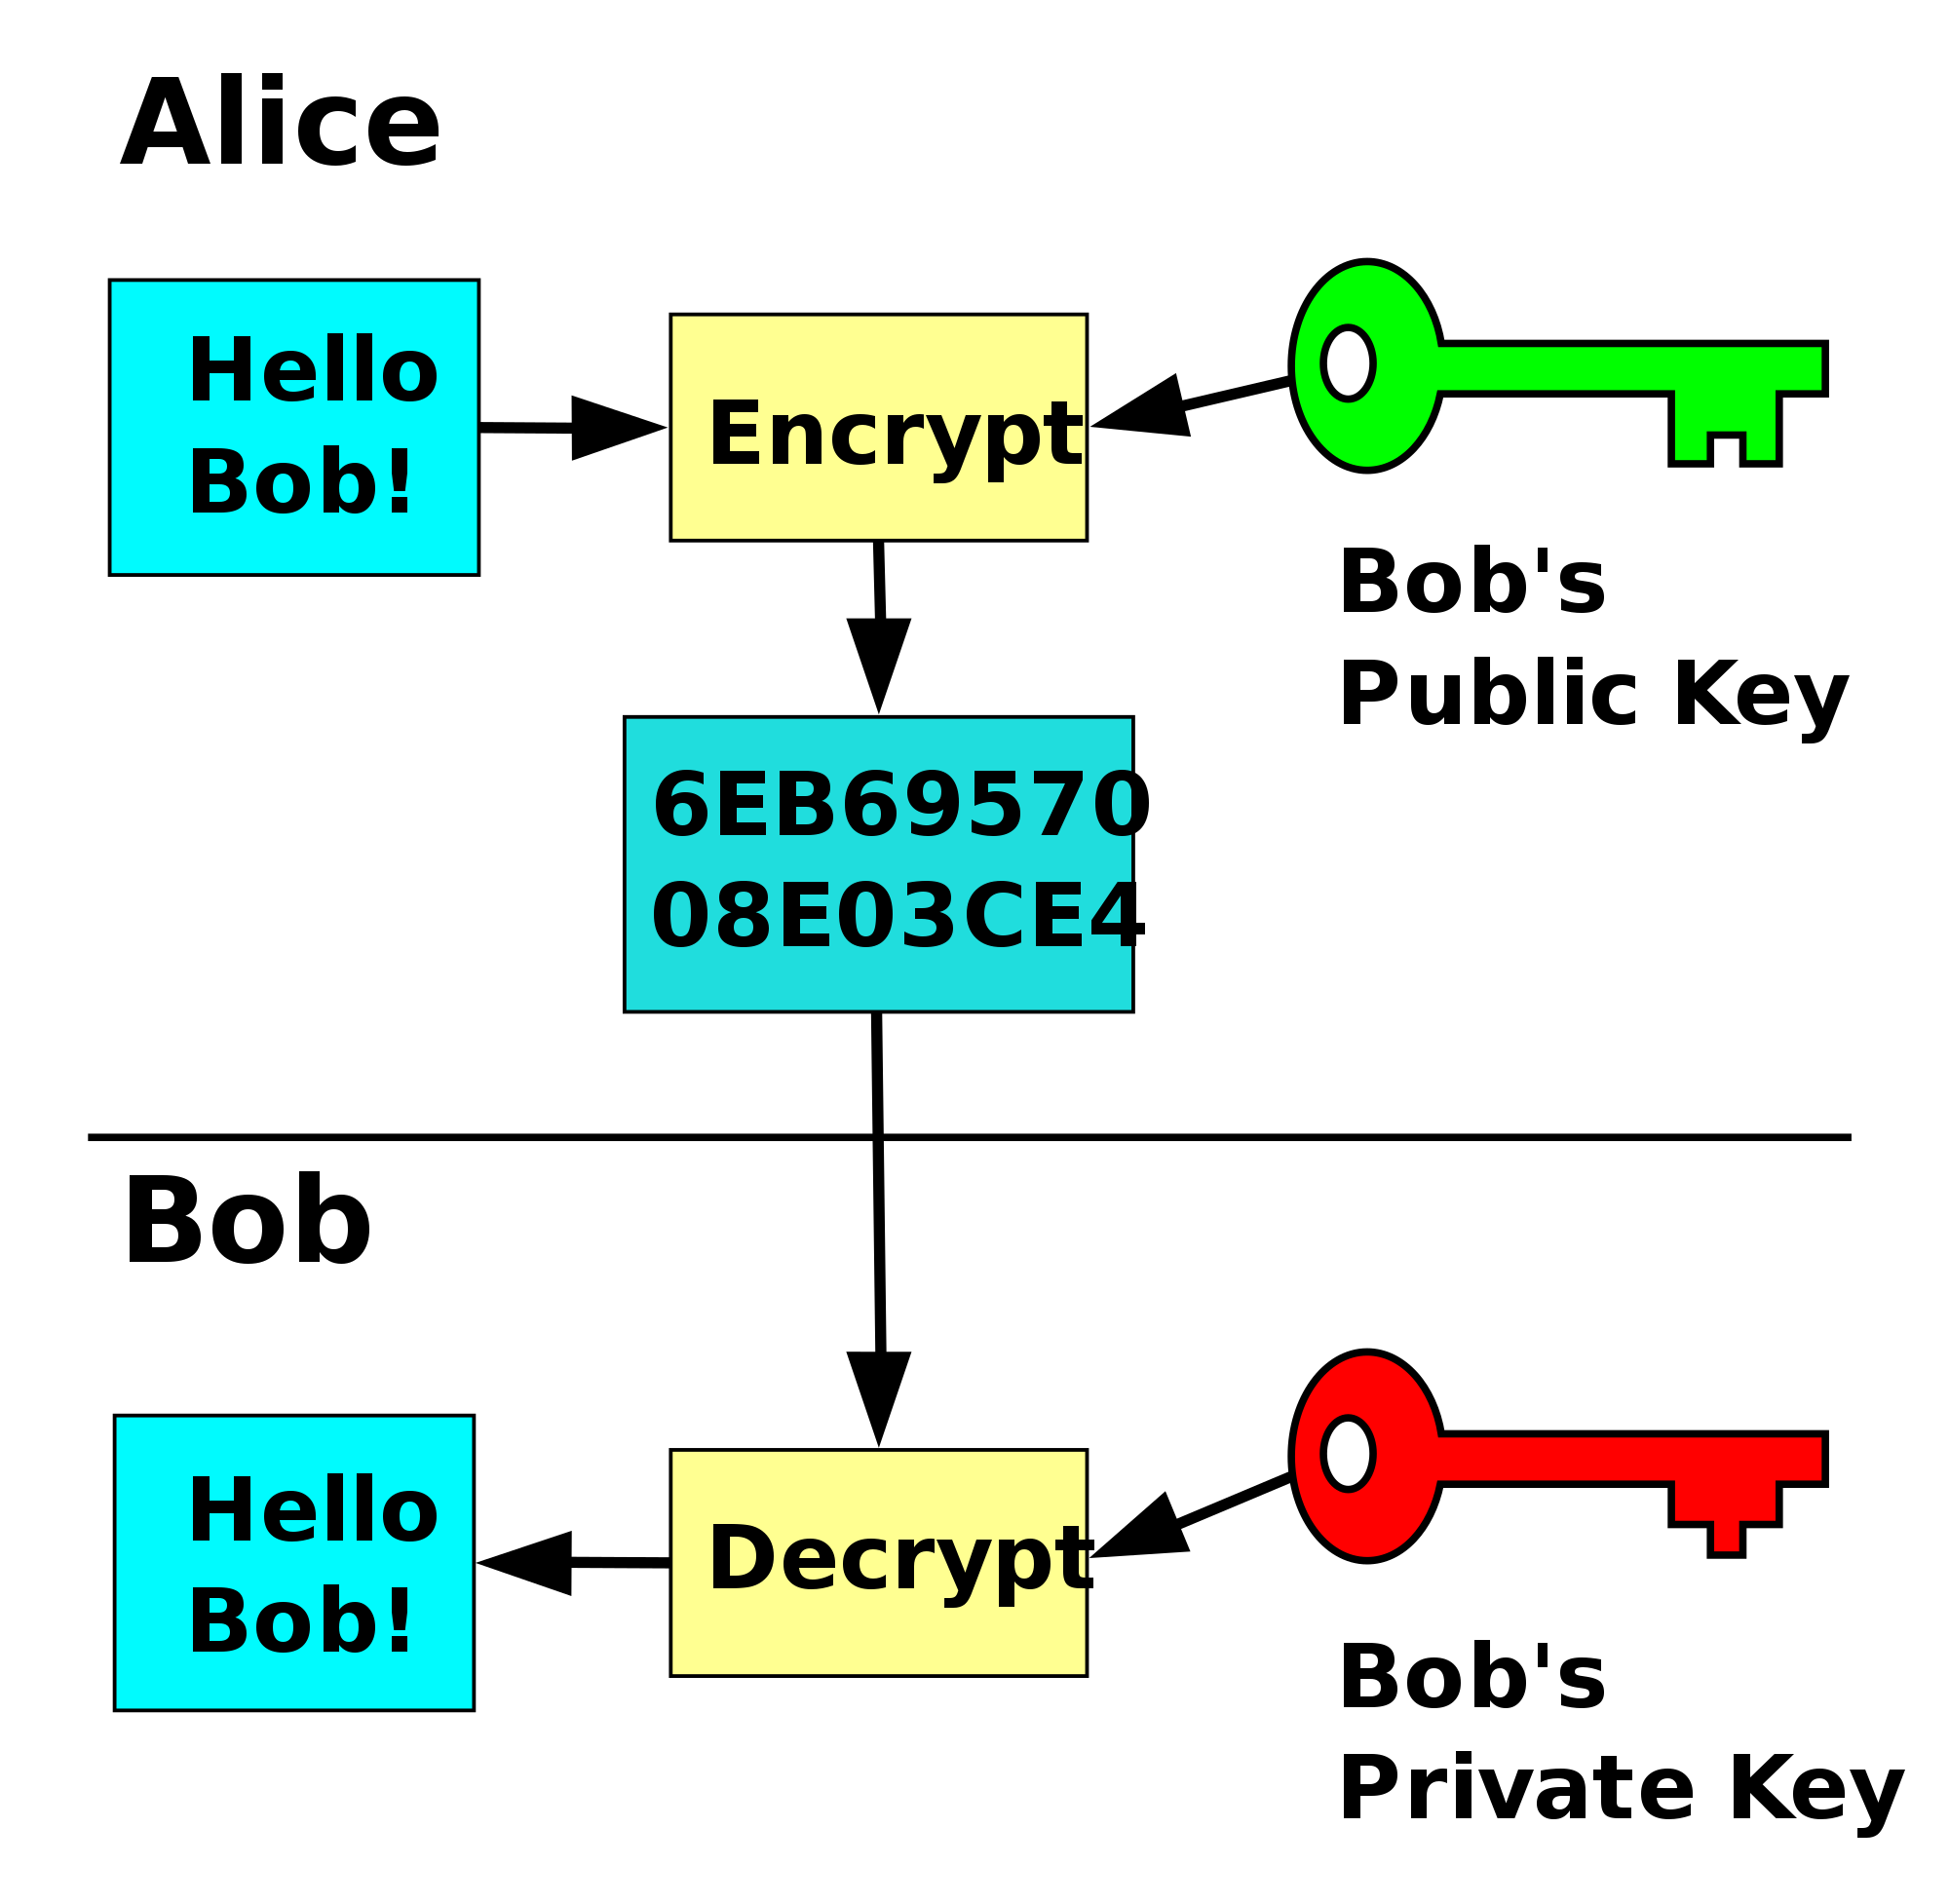
\includegraphics[scale=0.1]{./figures/Public_key_shared_secret.png}
            \end{center}
        \end{column}
    \end{columns}
\end{frame}

\begin{frame}
    \frametitle{Public Key Crypto: Digital Signature}
    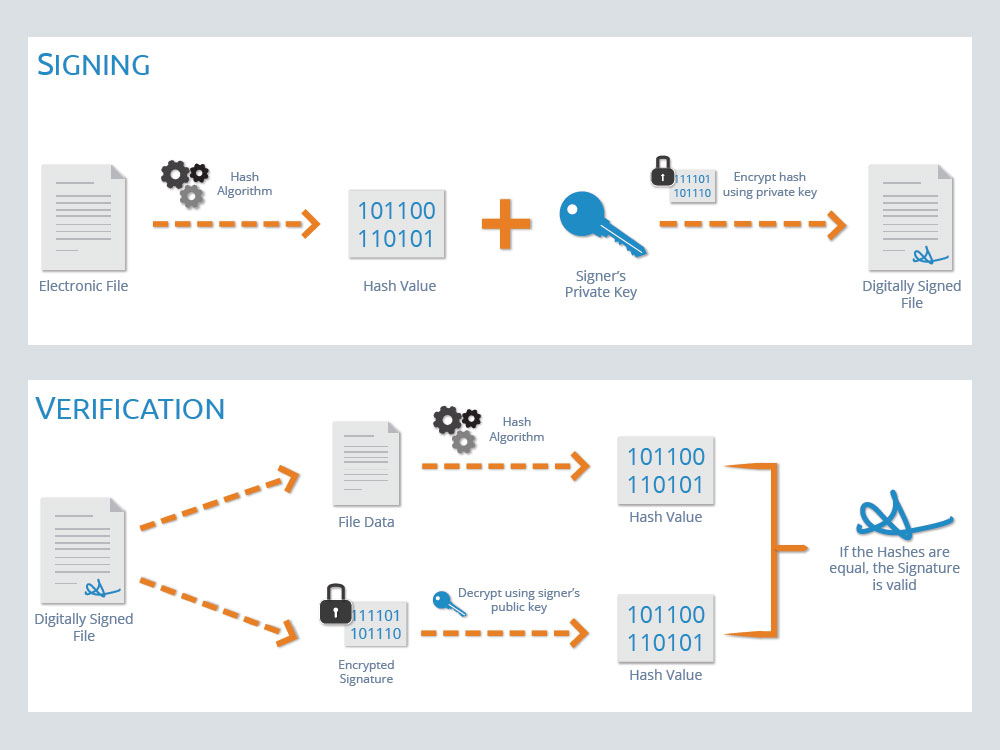
\includegraphics[scale=0.3]{./figures/digital-signatures-methodology.jpg}
\end{frame}

